\documentclass[11pt]{article}

\usepackage[utf8]{inputenc}
\usepackage[T1]{fontenc}
\usepackage{amsmath, amssymb}
\usepackage{geometry}
\usepackage{booktabs}
\usepackage{listings}
\usepackage{xcolor}
\usepackage{hyperref}
\usepackage{enumitem}
\usepackage{tikz}
\usetikzlibrary{positioning, arrows.meta}

\geometry{margin=1in}

\definecolor{codebg}{rgb}{0.96,0.96,0.96}
\lstset{
  backgroundcolor=\color{codebg},
  basicstyle=\ttfamily\small,
  breaklines=true,
  frame=single,
  language=Python,
  showstringspaces=false,
  columns=fullflexible,
  keywordstyle=\color{blue!70!black}
}

\newcommand{\diver}{\nabla\!\cdot}
\newcommand{\grad}{\nabla}
\newcommand{\bx}{\mathbf{x}}
\newcommand{\bp}{\mathbf{p}}
\newcommand{\R}{\mathbb{R}}

\title{RBF-FD Solver: Code Structure and Workflow}
\author{Dennis Corraliza}
\date{6/21/2026}

\begin{document}
\maketitle

\begin{abstract}
This note describes the structure of the RBF-FD (Radial Basis
Function Finite Difference) PDE solver implemented in
\texttt{assembly.py}, \texttt{domain.py}, \texttt{rbf.py},
\texttt{boundary.py}, \texttt{stencils.py}, and \texttt{geometry.py}.
It walks through the pipeline from node generation to solved nodal
values, module by module, with just enough mathematics to explain
\emph{why} each step exists. For the full derivation of the underlying
RBF-FD numerics, see the companion theory note.
\end{abstract}

\tableofcontents

%==============================================================
\section{What the solver computes}
%==============================================================

Given a domain $\Omega$ (a square or a disk), a diffusion tensor $A$,
a source term $f$, and boundary data, the solver produces an
approximate solution $u$ to
\[
  -\diver(A\grad u) = f \ \text{ in } \Omega,
\]
with Dirichlet conditions ($u$ prescribed) and/or Neumann conditions
($\partial u/\partial n$ prescribed) on different parts of the
boundary. It does this by:
\begin{enumerate}[leftmargin=2em]
  \item scattering nodes over $\Omega$,
  \item building, for each node, a small local stencil of nearby nodes,
  \item fitting local differentiation weights at each node so that a
        weighted sum of neighboring values approximates the PDE
        operator there,
  \item assembling all the local weights into one big sparse-like
        (here, dense) matrix $W$,
  \item overwriting the boundary rows of $W$ to enforce the boundary
        conditions,
  \item solving the resulting linear system $Wu = F$.
\end{enumerate}
The rest of this note walks through which file and function does each
step.

%==============================================================
\section{Module map}
%==============================================================

\begin{center}
\begin{tabular}{@{}ll@{}}
\toprule
\textbf{Module} & \textbf{Responsibility} \\
\midrule
\texttt{geometry.py} & Generates node coordinates for a given domain shape. \\
\texttt{stencils.py} & Builds nearest-neighbor stencils for every node. \\
\texttt{rbf.py} & Kernel functions, their gradients, and the (anisotropic) \\
                & Laplacian applied to each kernel; auxiliary grid generation. \\
\texttt{boundary.py} & Classifies nodes as interior/Dirichlet/Neumann; supplies \\
                      & boundary values and outward normals. \\
\texttt{domain.py} & \texttt{PDEDomainContext}: a plain data container holding \\
                    & everything (nodes, stencils, kernel choice, $A$, $W$, $F$, \dots). \\
\texttt{assembly.py} & The actual RBF-FD machinery: local weight solves, global \\
                      & assembly, boundary imposition, and the top-level driver. \\
\bottomrule
\end{tabular}
\end{center}

%==============================================================
\section{Pipeline diagram}
%==============================================================

\begin{center}
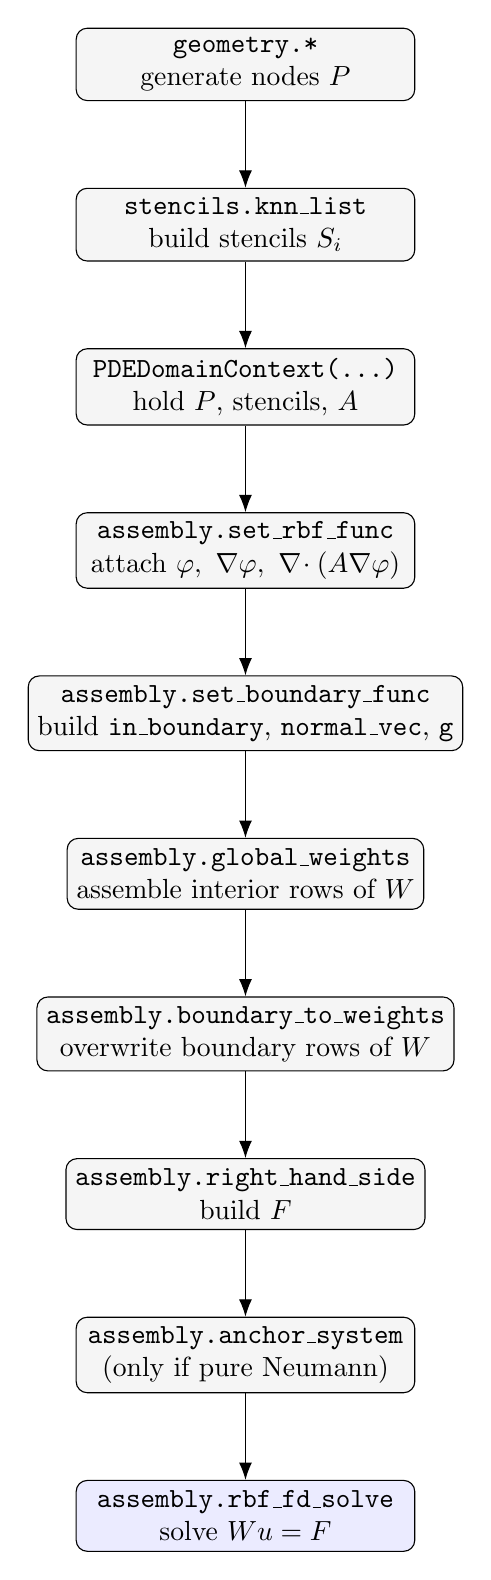
\begin{tikzpicture}[
  node distance=1.1cm and 0.4cm,
  box/.style={draw, rounded corners, align=center, minimum width=4.3cm,
              minimum height=0.9cm, fill=codebg},
  arr/.style={-{Latex[length=2.2mm]}}
]
\node[box] (geo)  {\texttt{geometry.*}\\generate nodes $P$};
\node[box, below=of geo] (sten) {\texttt{stencils.knn\_list}\\build stencils $S_i$};
\node[box, below=of sten] (ctx) {\texttt{PDEDomainContext(...)}\\hold $P$, stencils, $A$};
\node[box, below=of ctx] (rbfset) {\texttt{assembly.set\_rbf\_func}\\attach $\varphi,\ \grad\varphi,\ \diver(A\grad\varphi)$};
\node[box, below=of rbfset] (bset) {\texttt{assembly.set\_boundary\_func}\\build \texttt{in\_boundary}, \texttt{normal\_vec}, \texttt{g}};
\node[box, below=of bset] (gw) {\texttt{assembly.global\_weights}\\assemble interior rows of $W$};
\node[box, below=of gw] (b2w) {\texttt{assembly.boundary\_to\_weights}\\overwrite boundary rows of $W$};
\node[box, below=of b2w] (rhs) {\texttt{assembly.right\_hand\_side}\\build $F$};
\node[box, below=of rhs] (anchor) {\texttt{assembly.anchor\_system}\\(only if pure Neumann)};
\node[box, below=of anchor, fill=blue!8] (solve) {\texttt{assembly.rbf\_fd\_solve}\\solve $Wu=F$};

\draw[arr] (geo) -- (sten);
\draw[arr] (sten) -- (ctx);
\draw[arr] (ctx) -- (rbfset);
\draw[arr] (rbfset) -- (bset);
\draw[arr] (bset) -- (gw);
\draw[arr] (gw) -- (b2w);
\draw[arr] (b2w) -- (rhs);
\draw[arr] (rhs) -- (anchor);
\draw[arr] (anchor) -- (solve);
\end{tikzpicture}
\end{center}

All of these steps (except node generation and the final solve) are
chained together for you by \texttt{assembly.rbf\_fd\_system(\dots)},
which is the function most user code should actually call.

%==============================================================
\section{Step 1: Node generation (\texttt{geometry.py})}
%==============================================================

Four node-generation strategies are provided. They all return a plain
array $P \in \R^{N\times 2}$ of node coordinates; nothing downstream
cares how $P$ was produced.

\begin{itemize}[leftmargin=2em]
  \item \texttt{uniform\_square(L, Nx, Ny)} -- regular grid, boundary
        and interior points mixed together.
  \item \texttt{uniform\_int\_square(L, Nx\_int, Ny\_int, Nb)} -- regular
        interior grid, plus $N_b$ points per edge on the boundary,
        with corners de-duplicated. Returns \texttt{(P, num\_interior)}.
  \item \texttt{cheby\_square(L, Nx, Ny)} -- Chebyshev--Gauss--Lobatto
        points, clustered near the edges (standard for spectral
        methods).
  \item \texttt{circular\_geometry(R, Nx, Ny, num\_bound)} -- grid
        points filtered to the interior of a disk, plus points placed
        exactly on the circle.
\end{itemize}

\begin{lstlisting}
P, num_int = geometry.uniform_int_square(L=1.0, Nx_int=40, Ny_int=40, Nb=80)
\end{lstlisting}

%==============================================================
\section{Step 2: Stencils (\texttt{stencils.py})}
%==============================================================

For each node $\bx_i$, \texttt{stencils.knn\_list(P, k\_s)} finds the
$num_stencil_nodes$ nearest neighbors of $\bx_i$ (including itself) by Euclidean
distance, and returns a list \texttt{stencils[i]} of their indices in
$P$. This list is the only thing that determines which other nodal
values can contribute to the discrete operator at $\bx_i$.

%==============================================================
\section{Step 3: The domain context (\texttt{domain.py})}
%==============================================================

\texttt{PDEDomainContext} is a plain container, not a solver --- it
just holds state so functions in \texttt{assembly.py} don't need ten
positional arguments each. It is built once, then configured
incrementally with several \texttt{set\_*} calls:

\begin{lstlisting}
context = domain.PDEDomainContext(P, stencils, A)
context.set_phi(...)
context.set_grad_phi(...)
context.set_laplacian_phi(...)
context.set_augmentation(True)   # optional
context.set_centers(num_rings)         # optional: enables least-squares weights
\end{lstlisting}

By the end of the pipeline it also holds the assembled weight matrix
(\texttt{context.W}) and right-hand side (\texttt{context.F}), set via
\texttt{set\_W} / \texttt{set\_rhs}.

%==============================================================
\section{Step 4: Choosing a kernel (\texttt{rbf.py})}
%==============================================================

Two radial kernels are available, selected by the string
\texttt{basis} passed to \texttt{assembly.set\_rbf\_func}:

\begin{center}
\begin{tabular}{@{}lll@{}}
\toprule
\textbf{\texttt{basis}} & \textbf{Kernel $\varphi(\bp)$} & \textbf{Functions} \\
\midrule
\texttt{'cubic'} & $\|\bp\|^3$ & \texttt{phi\_cubic}, \texttt{grad\_phi\_cubic}, \\
                  & & \texttt{anisotropic\_diffusion\_phi\_cubic} \\
\texttt{'gaussian'} & $\exp(-(\varepsilon\|\bp\|)^2)$ & \texttt{phi\_gauss}, \texttt{grad\_phi\_gauss}, \\
                     & & \texttt{anisotropic\_diffusion\_phi\_gauss} \\
\bottomrule
\end{tabular}
\end{center}

The \texttt{anisotropic\_diffusion\_phi\_*} functions evaluate
$\diver(A\grad\varphi)$ in closed form (not numerically); this is what
makes the RBF-FD weights exact for the kernel rather than an
approximation of one. If \texttt{augmentation=True}, the linear
polynomial basis $\{1,x,y\}$ (\texttt{poly\_basis}, \texttt{grad\_poly},
\texttt{anisotropic\_diffusion\_poly}) is also added, so that the
local fit reproduces constants and linear functions exactly.

%==============================================================
\section{Step 5: Choosing a domain shape (\texttt{boundary.py})}
%==============================================================

\texttt{assembly.set\_boundary\_func} dispatches on the string
\texttt{shape} (\texttt{'square'} or \texttt{'circle'}) to build three
closures:

\begin{center}
\begin{tabular}{@{}lll@{}}
\toprule
& \textbf{square} & \textbf{circle} \\
\midrule
classify node & \texttt{in\_square\_boundary} & \texttt{in\_circular\_boundary} \\
outward normal & \texttt{square\_normal} & \texttt{disk\_normal} \\
boundary value & \texttt{square\_boundary} & \texttt{circular\_boundary} \\
\bottomrule
\end{tabular}
\end{center}

For the square, boundary data is supplied as a list of four
one-variable functions \texttt{[g1, g2, g3, g4]} for the bottom,
right, top, and left edges respectively (ordered counterclockwise
starting at $y=0$); for the disk, a single function \texttt{g(p)}
covers the whole boundary circle.

%==============================================================
\section{Steps 6--8: Assembly (\texttt{assembly.py})}
%==============================================================

\subsection{Local weight solves}

For each node, \texttt{local\_weights\_solve} (or, if
\texttt{context.center\_rings} is set, \texttt{local\_weights\_ls})
computes the row of differentiation weights for that node's stencil.
\texttt{local\_grad\_solve} / \texttt{local\_grad\_ls} do the same for
the gradient, needed only at Neumann boundary nodes. These four
functions are the computational core of the method; everything else
in \texttt{assembly.py} is bookkeeping around them.

\subsection{Global assembly}

\begin{lstlisting}
W = assembly.global_weights(context, in_boundary, normal_vec)
assembly.boundary_to_weights(W, context, in_boundary, normal_vec)  # in-place
F = assembly.right_hand_side(context, f, g, in_boundary)
\end{lstlisting}

\texttt{global\_weights} loops over every node and scatters its local
weights into a dense $N\times N$ matrix $W$. \texttt{boundary\_to\_weights}
then overwrites, in place, the rows of $W$ corresponding to Dirichlet
nodes (identity row) and Neumann nodes (directional-derivative row).
\texttt{right\_hand\_side} fills $F$ with $f$ at interior nodes and the
boundary data at boundary nodes.

\subsection{Pure-Neumann anchoring}

If every boundary node is Neumann (checked by
\texttt{is\_pure\_neumann}), $W$ is singular (the solution is only
determined up to a constant), so \texttt{anchor\_system(W, F, method)}
regularizes it using one of three strategies (\texttt{'mean'},
\texttt{'pin'}, or \texttt{'project'}) before solving.

%==============================================================
\section{Step 9: Solving (\texttt{assembly.rbf\_fd\_solve})}
%==============================================================

\begin{lstlisting}
u = assembly.rbf_fd_solve(context.W, context.F)
\end{lstlisting}
A thin wrapper around \texttt{numpy.linalg.solve}: nothing
RBF-FD-specific happens here, since all of the discretization work was
already baked into $W$ and $F$.

%==============================================================
\section{Putting it together: the top-level driver}
%==============================================================

In practice, a user only needs to call:

\begin{lstlisting}
context = assembly.rbf_fd_system(
    f, g_bound, btype, P,
    basis='cubic', shape='square', L=1.0,
    num_stencil_nodes=25, num_rings=None,        # num_rings=None -> direct solve; num_rings=int -> least squares
    augmentation=True, A=my_tensor
)
u = assembly.rbf_fd_solve(context.W, context.F)
\end{lstlisting}

\texttt{rbf\_fd\_system} runs steps 3 through 8 end-to-end (printing a
short progress message after each stage) and returns a fully populated
\texttt{PDEDomainContext}, ready to be handed to \texttt{rbf\_fd\_solve}.

%==============================================================
\section{Validating the solver: manufactured solutions}
%==============================================================

To check that the solver is actually correct, test problems are
built by picking a closed-form $u_{\text{exact}}$, then differentiating
it analytically to obtain a matching $f$ and boundary data --- this is
the \emph{method of manufactured solutions}. Each such test problem is
a small Python function (e.g.\ \texttt{example\_3}) returning the
tuple \texttt{(f, g, btype, u\_exact)}, ready to be passed straight into
\texttt{rbf\_fd\_system}. Once solved, \texttt{report\_and\_graph(context,
u\_exact)} compares the numerical solution against $u_{\text{exact}}$
at every node and reports:

\begin{itemize}[leftmargin=2em]
  \item the condition number of $W$,
  \item the maximum pointwise error and a discrete $L^2$ error,
  \item contour and 3D surface plots of the approximate solution, the
        exact solution, and the pointwise error.
\end{itemize}

This is the standard way to sanity-check a new kernel, stencil size,
or boundary condition setup before trusting the solver on a problem
without a known exact solution.

\end{document}
